%!TEX root = ../crimson_throne_book_main.tex
% 2015-03-28
Finally ... finally ... With a mixture of relief and sadness Balian tries to come to grips with what just happened. Yes, after five years he has finally found his sister; after five years he has finally tracked down the bastard who took his dear Alika from him and yes ... the foul kidnapper did not get away. But half a decade is a long time, the vicious necromancer got under her skin, he brainwashed her, changed her, molded her into his equally vicious right-hand woman. Looking at her now, as she's being bound and gagged, Balian sees nothing but hatred in her eyes. Only Spyder treats her as if nothing has changed, clinging to her side and rubbing his head against her leg. The ranger calls his dog over. The animal gives him a sad puppy look, quickly licks Alika's hand before hesitantly trotting to his master's feet.\\

Puk finds a key ring with a set of heavy keys next to the door in the back of the room. It opens into a small cellblock, which still holds three prisoners. One of them is dead, one unconscious and one barely alive. All three display heavy symptoms of the plague. Sjo offers the two living ones, a boy and a young woman, a {\itshape lesser restoration} to restore some of their stamina. The boy recognizes the healer, he is a stable boy from the Great Tower, the headquarters of the Sable Company, where Sjo used to work as well. His name is Dalvun. He explains that he and his other cellmates have been used in experiments, they were frequently made to drink foul water by Doctor Saulus, Rolth, Alika and Lady Andaisin. Most of them are dead now. Only he and Jaelle are still alive. The two survivors are told to wait in the cultists' barracks, while the unconscious enemies are locked behind bars now. Sjo tells Dalvun he will be back soon, but first he and his friends have to take care of the evil priestess. Returning to the room with the skeletal bacchanal of Urgathoa decorating the walls, the companions now take the heavy metal door deeper into the complex. The stinging scent of chemicals greets them. A huge basin, filled to the brim with foul, murky water, dominates the center of this high-ceilinged chamber. Two sets of stairs to the left and right lead to a catwalk ten feet above the ground which stretches over the pool. Two cultists are inside, one of them stands at the back of the room in an open door. "Warn our Lady that the intruders have arrived!" he yells to someone in the room beyond, before shutting the door. The other cultist is up on the catwalk. Puk, Spyder and Sjo make quick work of the first one, while Balian storms up the stairs and engages the cultist on the overpass. His heavy blade sinks deep into the poor man's shoulder. The ranger pulls his sword free and cleaves the Urgathoan devotee in two: his legs drop down on the metal walkway, while his torso plummets in the foul water below. A fitting end for one who worships a goddess whose upper and lower body are so distinctly separated.\\

The companions decide not to waste any time and ignore the doors to the left and right for now, choosing to follow the shouted warning and explore the way ahead first. The door opens into a hall with four large, cylindrical glass vats, each filled with a bubbling emerald fluid that tints the chamber's light a noxious green. Within each container floats a malformed abomination - part man and part horse - a lean, leathery male body resting on a horse's hind legs and topped with a fleshless equine skull. Three of these forms drift motionless in the green bile, but the fourth still twitches. An alarmed cultist is standing next to the fourth vat and smashes the glass to pieces, spilling the vile liquid over the floor and freeing the creature within. Balian and Puk charge the man and cut him down, but are greeted by the abomination, which lowers its jaw bone, spreading its mouth wide: a swarm of corpse-bloated black flies spills forth from its beak, biting and sickening the two unfortunates. Quint and Sjo resort to combat healing to keep their mates afoot, while\hyperref[fig:Leukodaemon-523050841]{ the daemon now starts clawing and chawing at all those within its reach } . The companions lure the creature away from the corner, so they can surround it and start cutting it up one gash at a time. Their combined attacks quickly outpace the creature's offensive and a few moments later the giant harbinger of disease lies dead at their feet. \\

\begin{figure}[h]
	\centering
	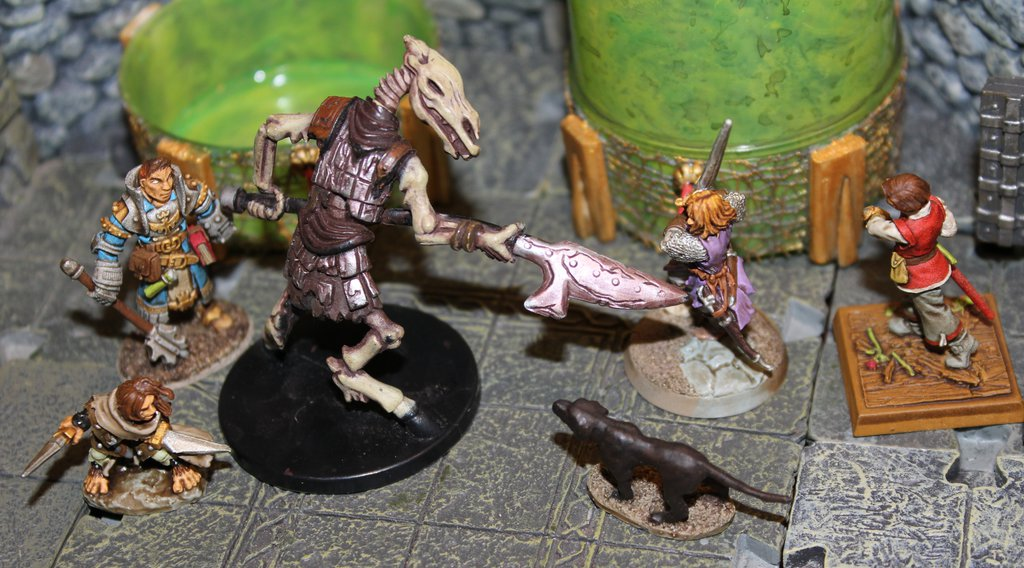
\includegraphics[width=0.39\textwidth]{images/Leukodaemon-523050841.jpg}
	\caption{Leukodaemon}
	\label{fig:Leukodaemon-523050841}
\end{figure}

